\section{Curl-closure ontology}\label{sec:curl-closure-ontology}

This section uses the curl-closure names fixed in \apref{app:cc-naming-conventions}. The names are ontological roles inside the fractal tesseract topology.

\begin{definition}[Curl motif / closure witness. \apref{app:cc-curl}]
Curl is the Stokes-aligned circulation/closure witness on the cited support. AOD records its retained cut dynamics as hinge return, reclosure, duration, orientation, and returned-current bookkeeping on declared windows. It distinguishes outgoing side, hinge, returned side, closure point, duration, and orientation.
\end{definition}

\begin{definition}[Nested curl. \apref{app:cc-nested-curl}]
A nested curl is a curl carried inside another curl. It distinguishes inner return, outer return, and the hinge by which the inner return re-enters the outer closure.
\end{definition}

\begin{definition}[Pin-curl. \apref{app:cc-pin-curl}]
A pin-curl is a returned curl whose residue seats, delays, or fixes a hinge. Pinning makes a curl persist across later return.
\end{definition}

\begin{definition}[Curling curls. \apref{app:cc-curling-curls}]
Curling curls are recursive returns that become active path structure inside the fractal tesseract topology.
\end{definition}

The relation chain is
\[
\text{return through hinge}\to \text{curl}\to \text{nested curl}\to \text{pin-curl}\to \text{curling curls}.
\]

\begin{definition}[Memorum]
The memorum is the retained temporal structure of an observer-field:
\[
\mathcal M=(\text{predecessor closure},\ \text{present boundary},\ \text{successor horizon}).
\]
It keeps predecessor retention, present boundary, and successor horizon available to the same closure.
\end{definition}

\begin{definition}[Monon. \apref{app:cc-monon}]
A monon is the primitive completed cycle of \(x\succ x=x\): null symmetry presents asymmetric cut-running, the cut reflects as duration, and the reflected duration closes on the declared return:
\[
\mathrm{monon}(x)=\operatorname{cycle}(x\succ x=x).
\]
\end{definition}

\begin{definition}[Dion. \apref{app:cc-dion}]
A dion is the first two-position return curl around the monon hinge. The two oriented dion returns are
\[
D_\alpha=(+1,-1),\qquad D_\Omega=(-1,+1).
\]
\end{definition}

\begin{definition}[Duon. \apref{app:cc-duon-duad-wavelet}]
A duon is two dion returns coupled through one carried monon seat:
\[
\mathrm{duon}=D_i\Box D_j,
\qquad D_i,D_j\in\{D_\alpha,D_\Omega\}.
\]
A resolved duon carries a monon pivot value:
\[
D_i\mu D_j,
\qquad \mu\in\{-1,0,+1\}.
\]
\end{definition}

\begin{definition}[Duad. \apref{app:cc-duon-duad-wavelet}]
A duad is the seat-taken state of the same duon current.
\end{definition}

\begin{definition}[Trion, tetrion, tetron, tetratrion. \apref{app:cc-tetrion-tetron-tetratrion}]
A trion is a three-phase internal knot. A tetrion is the bare four-cycle / four-pivot return closure. A tetron is \(E_4\): the default inner cage with four seats. A tetratrion is \(3:4=4\times\mathrm{trion}\). \apref{app:cc-tetrion-tetron-tetratrion}.
\end{definition}

\paragraph{Field-as-monon compression.}
When a declared boundary encloses a complete retained field \(\mathcal F\), the enclosed field can be bound as one monon cycle relative to the next enclosing address:
\[
\mathrm{monon}_{\mathcal F}=\operatorname{cycle}_{\partial\mathcal F}(x\succ x=x).
\]
The internal field may contain curls, shells, wavelet groups, returned-current duration, pressure, and PADAR. The enclosing boundary can still bind the whole field as one cycle.

\begin{figure}[H]
\centering
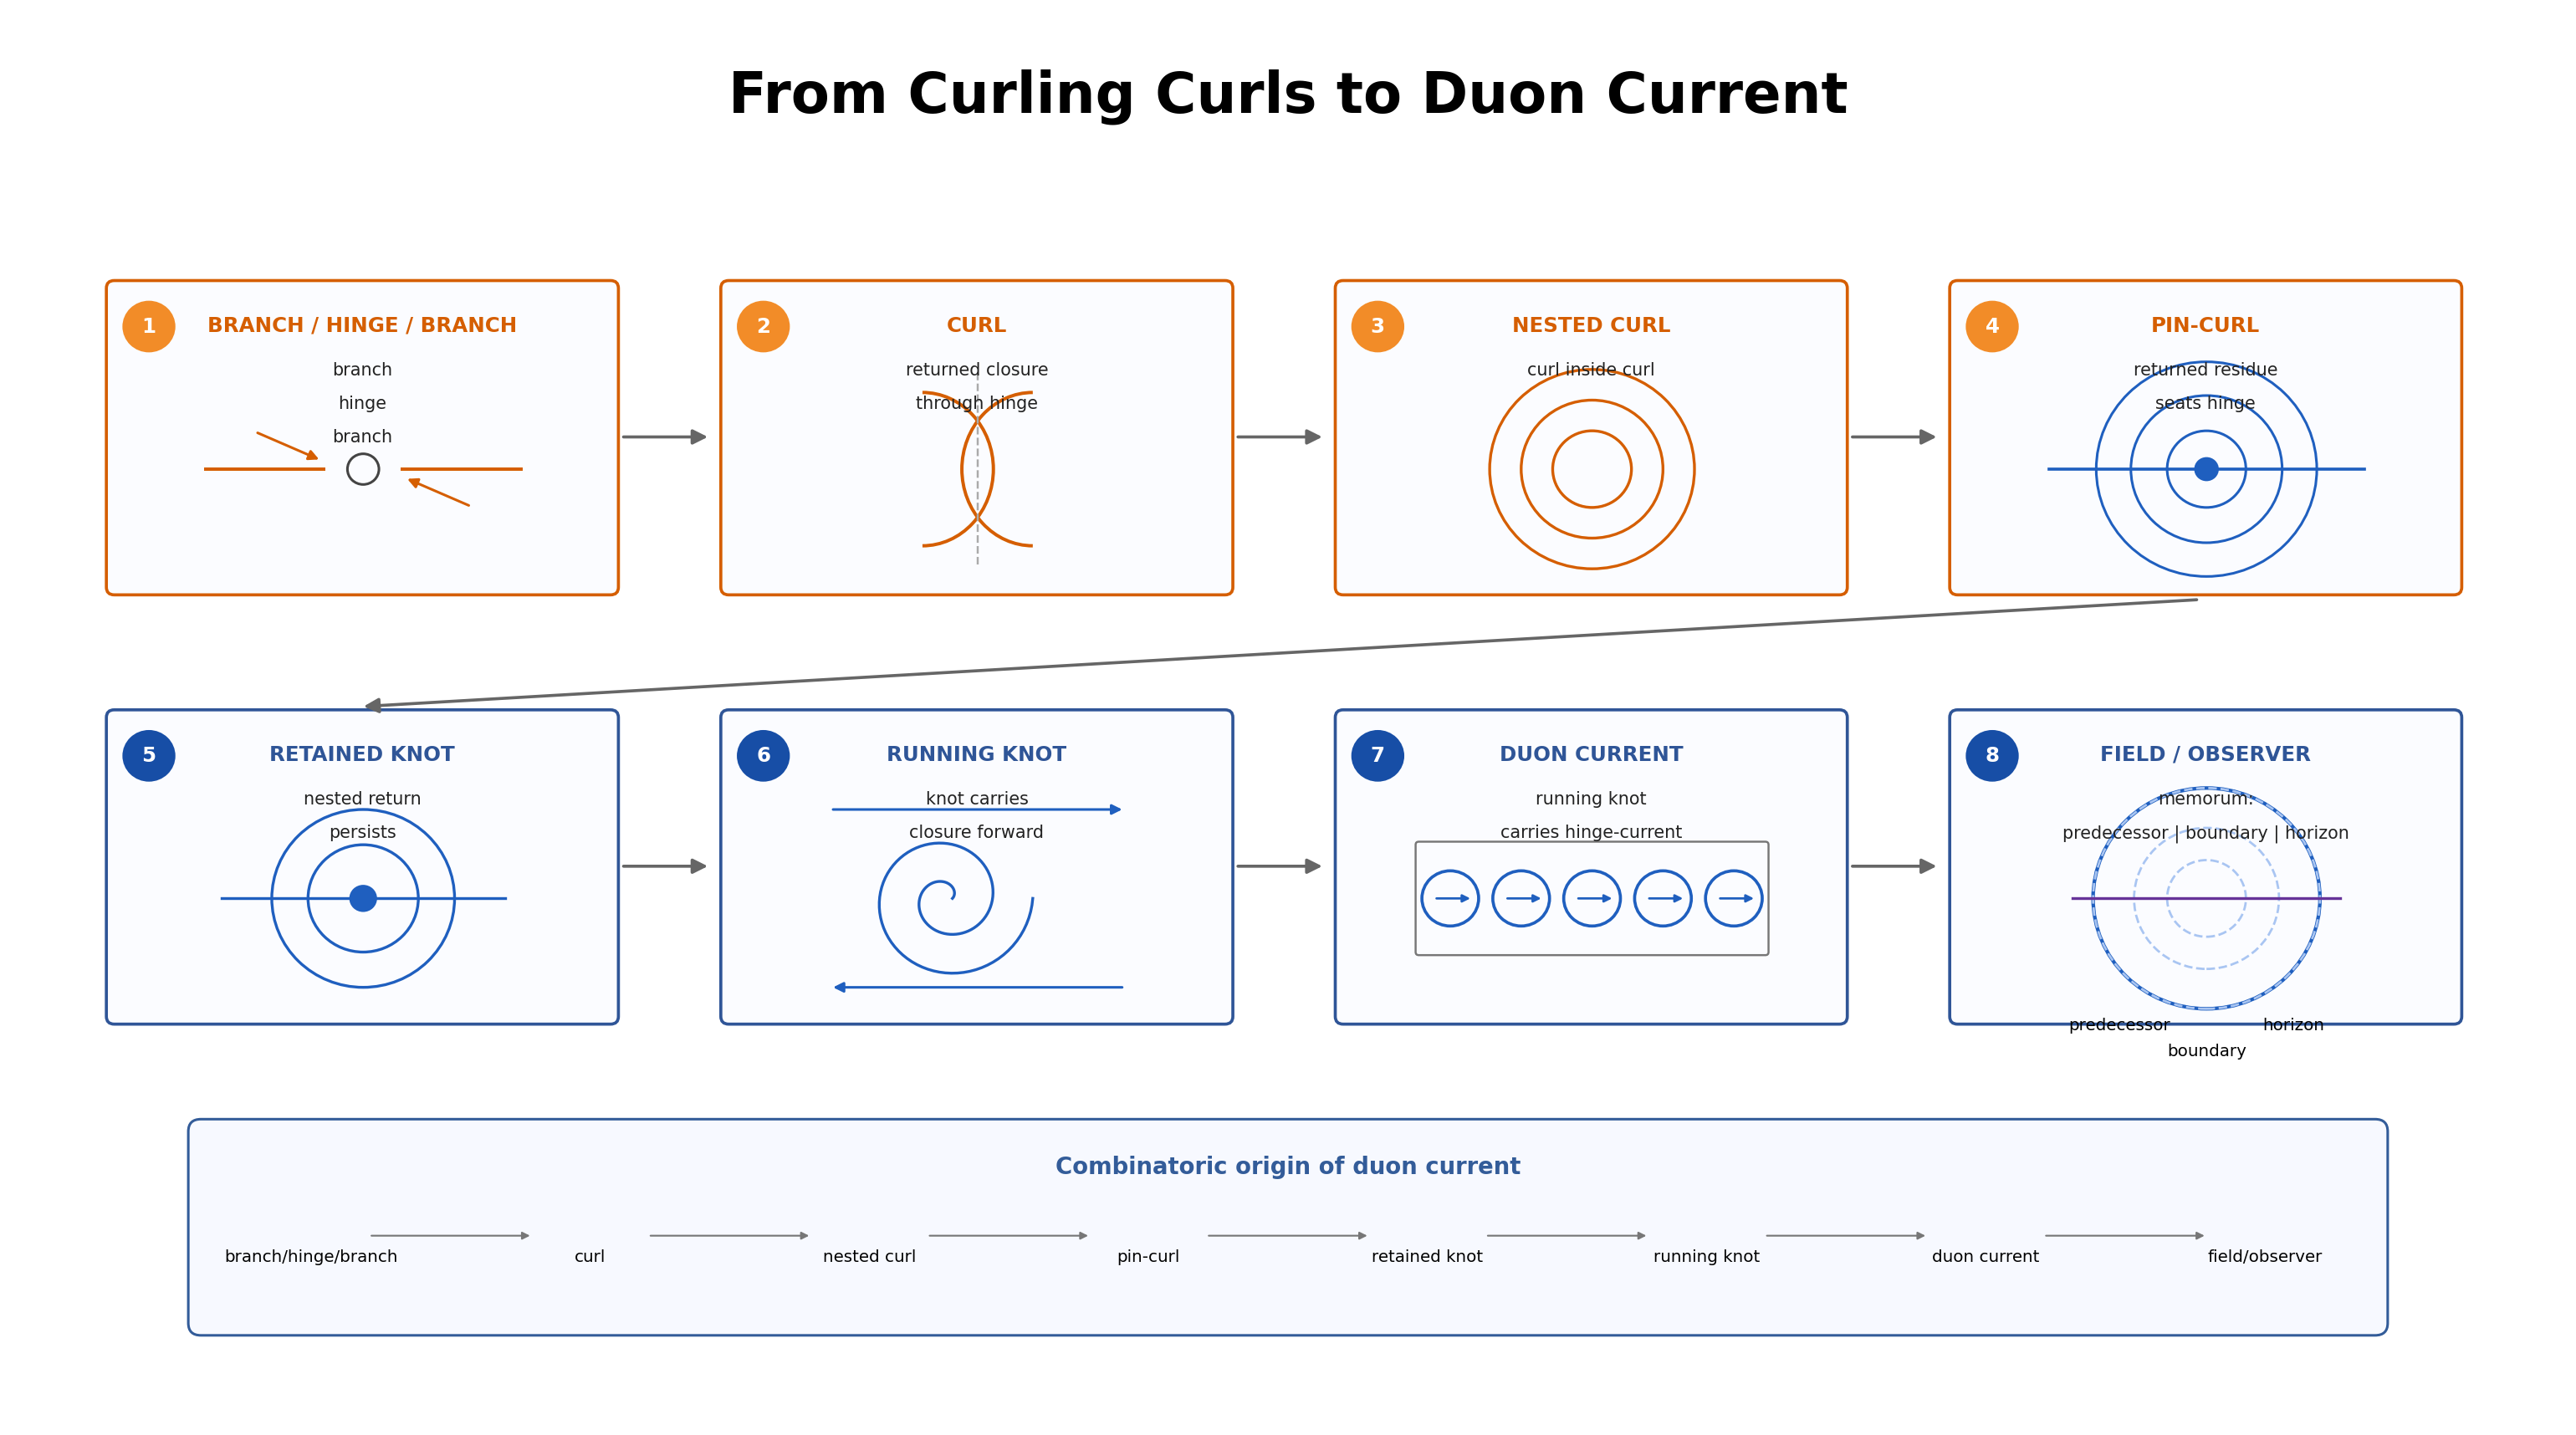
\includegraphics[width=0.96\linewidth]{figures_jpg/v39_15_curling_curls_to_duon_current_field_observer.png}
\caption{From curling curls to duon current. Branch/hinge/branch returns form curls; recursive curls become pin-curls, retained knots, running knots, duon current, and field/observer support.}
\label{fig:curling-curls-to-duon-current}
\end{figure}
